\section{Results}

\subsection{Compression and Random-Access Correctness}

The first question is whether the representation behaves like a genuine random-access format rather than only a compact storage blob. Across the verified serializer tests and real-trace evaluations, the container round trip preserved block-local reconstruction, and independently decoded blocks matched the corresponding slices of full reconstruction. This matters because the certificate is only operationally meaningful if the system can address a selected historical block without replaying earlier blocks. The random-access contract is therefore not merely a software invariant; it is part of the scientific claim that compression and selective use of history can coexist.

The same evidence also clarifies what has \emph{not} yet been shown. Independent logical decoding does not automatically imply lower runtime or lower bandwidth. The present experiments validate the storage and reconstruction contract itself. They do not claim that every independently addressable block is already being omitted physically in a deployed inference engine.

\subsection{Storage--Accuracy Tradeoff}

How much storage can the current block-local codec save while keeping local attention outputs close to the full-cache reference? In the representative-layer benchmark, RACK-KV reduced serialized KV storage from roughly \num{91.8}~kB for the reference serialization to roughly \num{56.2}~kB on average, corresponding to a mean savings of \num{36.5}\%. The mean attention-output error was \num{2.29e-3}. A separate longer layer-0 pilot at the same \(W=16\), \(B=8\) configuration reached a final-prefix storage reduction of roughly \num{40.4}\%, which is consistent with the representative-layer picture while remaining confined to a different experimental scope.

\begin{table}[t]
  \centering
  \small
  \begin{threeparttable}
\small
\hfuzz=1pt
\setlength{\tabcolsep}{3pt}
\begin{tabular*}{\linewidth}{@{\extracolsep{\fill}}l c c c c c c c@{}}
\toprule
Method & Cfg. & {\makecell{Bytes\\(kB)}} & {\makecell{Mean\\L2}} & {\makecell{Median\\L2}} & {\makecell{P95\\L2}} & Ratio & {\makecell{Saving\\(\%)}} \\
\midrule
Full KV & N & 91.8 & 0 & 0 & 0 & 0.99 & -0.7 \\
RACK-KV & N & 56.2 & $2.3 \times 10^{-3}$ & $8.3 \times 10^{-4}$ & $1.0 \times 10^{-2}$ & 1.58 & 36.5 \\
Uniform INT8 & N & 51.3 & $6.5 \times 10^{-3}$ & $5.1 \times 10^{-3}$ & $1.8 \times 10^{-2}$ & 1.73 & 41.5 \\
KIVI-style & N & 20.8 & $4.1 \times 10^{-1}$ & $3.0 \times 10^{-1}$ & $1.2$ & 4.13 & 73.1 \\
SnapKV-style & M & 56.2 & $1.2 \times 10^{-2}$ & $6.0 \times 10^{-3}$ & $4.9 \times 10^{-2}$ & 1.58 & 36.4 \\
Quest-style & M & 56.2 & $2.8 \times 10^{-2}$ & $1.6 \times 10^{-2}$ & $1.0 \times 10^{-1}$ & 1.59 & 36.9 \\
\bottomrule
\end{tabular*}
\begin{tablenotes}[flushleft]
\item N denotes the native configuration and M the matched-budget configuration. The negative saving for Full KV reflects small serialization overhead in the benchmark container rather than compression failure.
\end{tablenotes}
\end{threeparttable}

  \caption{Representative-layer comparison on \num{330} query cases. Matched-budget baselines target the serialized byte count of RACK-KV as closely as their discrete token or block choices allow.}
  \label{tab:mainresults}
\end{table}

\begin{figure}[t]
  \centering
  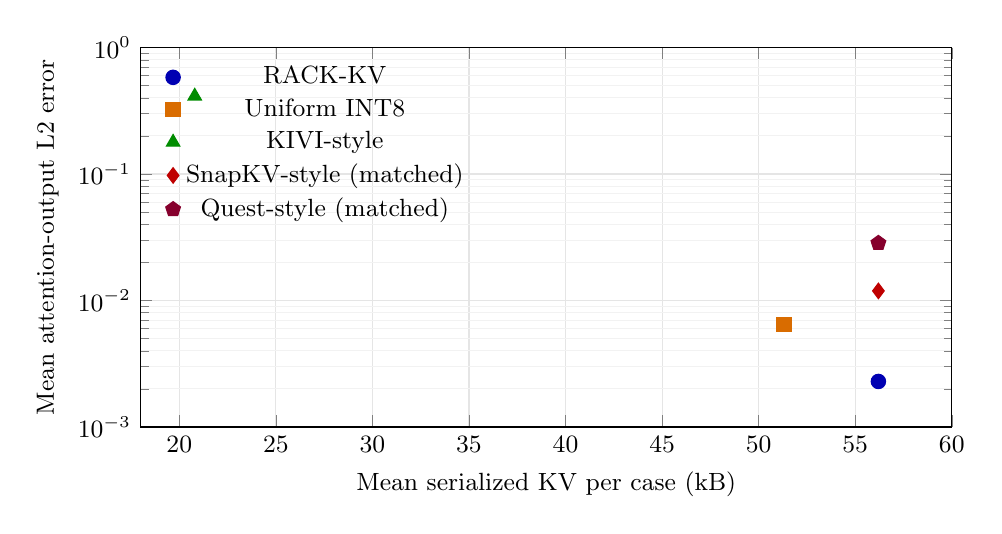
\begin{tikzpicture}
\begin{axis}[
  width=0.98\linewidth,
  height=6.4cm,
  xlabel={Mean serialized KV per case (kB)},
  ylabel={Mean attention-output L2 error},
  ymode=log,
  xmin=18,
  xmax=60,
  ymin=1e-3,
  ymax=1,
  grid=both,
  major grid style={gray!20},
  minor grid style={gray!10},
  legend style={draw=none, fill=none, font=\small, at={(0.02,0.98)}, anchor=north west},
  tick label style={font=\small},
  label style={font=\small}
]
  \addplot[only marks, mark=*, mark size=2.6pt, color=blue!70!black]
    coordinates {(56.2, 2.29e-3)};
  \addlegendentry{RACK-KV}

  \addplot[only marks, mark=square*, mark size=2.6pt, color=orange!85!black]
    coordinates {(51.3, 6.47e-3)};
  \addlegendentry{Uniform INT8}

  \addplot[only marks, mark=triangle*, mark size=2.8pt, color=green!55!black]
    coordinates {(20.8, 4.13e-1)};
  \addlegendentry{KIVI-style}

  \addplot[only marks, mark=diamond*, mark size=2.8pt, color=red!75!black]
    coordinates {(56.2, 1.19e-2)};
  \addlegendentry{SnapKV-style (matched)}

  \addplot[only marks, mark=pentagon*, mark size=2.8pt, color=purple!70!black]
    coordinates {(56.2, 2.84e-2)};
  \addlegendentry{Quest-style (matched)}
\end{axis}
\end{tikzpicture}

  \caption{Mean representative-layer attention-output error versus mean serialized KV size. Lower and further left is better. The full-cache reference is exact and therefore omitted from the log-scale error axis.}
  \label{fig:errorbytes}
\end{figure}

These numbers should not be interpreted as pure quantization performance. RACK-KV spends bytes on anchors, scales, indices, and geometric summaries because the representation is designed to support random access and later certification, not only compression. That overhead is visible in the comparison with Uniform INT8, which uses slightly fewer bytes on average. The more relevant question is whether the extra structure buys a better operating point once attention error is taken into account. On that criterion, it does: RACK-KV remains in a lower-error region than the more aggressive approximations at comparable storage scale.

\subsection{Matched-Budget Baseline Comparison}

The matched-budget comparison isolates the effect of representation quality from the effect of simply using more memory. At approximately the same serialized-memory budget, RACK-KV is more accurate than the selection-based baselines used here. SnapKV-style matching yields a mean error of \num{1.19e-2}, and Quest-style matching yields \num{2.84e-2}, both above RACK-KV's \num{2.29e-3}. The interpretation is consistent with the design of the methods: RACK-KV preserves historical information in compressed form and skips only when the certificate permits it, whereas selection baselines achieve the same budget partly by discarding some historical information outright.

The comparison with Uniform INT8 is subtler and scientifically more interesting. Uniform INT8 quantizes the whole eligible cache and therefore preserves all positions, but it does not exploit local sequence structure or block-level metadata. It uses somewhat fewer bytes than RACK-KV, yet its mean error is still about three times larger. This suggests that the added cost of anchors and block summaries is justified when the goal is not merely to shrink the cache, but to shrink it while preserving the attention computation more faithfully.

The KIVI-style baseline highlights the opposite extreme. In the project implementation it reaches a much stronger compression ratio, but at the cost of much larger attention-output distortion. That result should not be read as a claim about the original KIVI paper beyond the project scope. It does, however, illustrate the broader point that the most aggressive low-bit approximations can move the storage frontier much further left at the cost of a qualitatively different error regime.

\subsection{Certificate Safety}

The main empirical question for the theorem is safety: when the certificate authorizes a skip, does the observed local error remain below the certified upper bound? Across \num{6750} evaluated representative-layer candidate blocks, no rigorous violation, approximate violation, false-safe case, or numerical fallback was observed. The largest observed skipping error among skipped cases was approximately \num{3.26e-2}, while the largest rigorous upper bound was approximately \num{4.36e-2}. Within the evaluated scope, every observed skipped case remained below its bound.

\begin{table}[t]
  \centering
  \small
  \begin{threeparttable}
\begin{tabularx}{\linewidth}{@{}l c X@{}}
\toprule
Quantity & Result & Interpretation \\
\midrule
Evaluated block decisions & \num{6750} & Total candidate decisions examined in the representative-layer benchmark \\
Certified skips & \num{14} & Few blocks satisfied the current local bound \\
Weighted skip fraction & \num{0.21}\% & Safe but sparse certified skipping \\
Cases with any skip & \num{14}/\num{330} & Skips were concentrated in a small subset of cases \\
Rigorous violations & \num{0} & No skipped case exceeded its rigorous bound \\
False-safe cases & \num{0} & No block was skipped without empirical safety in the evaluated data \\
Numerical fallbacks & \num{0} & The multiprecision path did not require unresolved fallback handling \\
Largest observed skip error & \num{3.26e-2} & Maximum empirical deviation among skipped cases \\
Largest certificate bound & \num{4.36e-2} & Conservative upper bound remained above the observed maximum \\
Largest per-case skip fraction & \num{3.3}\% & Even the most aggressive skipped case remained modest \\
\bottomrule
\end{tabularx}
\end{threeparttable}

  \caption{Representative-layer certificate summary for RACK-KV. The key result is the absence of observed violations; the equally important limitation is the low certified skip rate.}
  \label{tab:cert}
\end{table}

This is the strongest theorem-related empirical result in the paper. It does not prove universal safety, but it does show that the implemented certificate behaves consistently with its theoretical role on real captured KV states. The absence of false-safe cases is especially important because RACK-KV is meant to be conservative. A theorem that skipped aggressively but occasionally authorized an unsafe omission would not serve the intended purpose.

\subsection{Certificate Tightness and Skip Frequency}

\begin{figure}[t]
  \centering
  \begin{tikzpicture}
\begin{axis}[
  width=0.98\linewidth,
  height=6.2cm,
  xlabel={Observed local skipping error},
  ylabel={Rigorous upper bound},
  xmin=0,
  xmax=0.045,
  ymin=0,
  ymax=0.045,
  grid=both,
  major grid style={gray!20},
  minor grid style={gray!10},
  tick label style={font=\small},
  label style={font=\small}
]
  \addplot[dashed, color=gray!70] coordinates {(0,0) (0.045,0.045)};
  \addplot[
    only marks,
    mark=*,
    mark size=2.2pt,
    color=blue!70!black
  ]
  table[
    col sep=comma,
    x=observed_skipping_error,
    y=certificate_upper_bound
  ]{data/stage4_rack_skip_cases.csv};
\end{axis}
\end{tikzpicture}

  \caption{Observed skipping error versus certified upper bound for the representative-layer cases that were actually skipped. Every point lies below the diagonal. The small number of points reflects the low skip rate rather than missing records.}
  \label{fig:boundobserved}
\end{figure}

Safety alone is not enough; a certificate that never skips is correct but unhelpful. The current bound skips rarely. Only \num{14} of the \num{6750} candidate block decisions were certified as skippable, corresponding to a weighted skip fraction of about \num{0.21}\%. This means that the current theorem is much more successful as a safety filter than as an aggressive compute-reduction mechanism.

The scatter in \Cref{fig:boundobserved} makes the same point geometrically. The observed errors stay below the bound, but the margin is not tiny. The present bound is therefore informative enough to certify a small number of decisions, yet loose enough that most candidates are retained. That pattern is consistent with the theoretical sources of conservativeness discussed in \Cref{sec:conservative}. The paper's evidence thus supports a careful conclusion: the certificate is empirically safe in the evaluated cases, but it is operationally conservative.

\subsection{Layer-Dependent Behavior}

The representative-layer benchmark also shows that reconstruction difficulty is not uniform across the Transformer stack. Even at a fixed storage budget, layers \(8\) and \(16\) are more sensitive under the current codec than layers \(0\) and \(24\), with layer \(31\) occupying an intermediate regime.

\begin{table}[t]
  \centering
  \small
  \begin{threeparttable}
\begin{tabular}{@{}c
S[scientific-notation=true,table-format=1.2e-1]
S[scientific-notation=true,table-format=1.2e-1]
S[scientific-notation=true,table-format=1.2e-1]
S[scientific-notation=true,table-format=1.2e-1]@{}}
\toprule
Layer & {Mean L2} & {Median L2} & {$95^{\mathrm{th}}$ pct.} & {Maximum} \\
\midrule
0  & 5.03e-4 & 3.74e-4 & 1.20e-3 & 2.66e-3 \\
8  & 3.84e-3 & 1.16e-3 & 1.38e-2 & 3.26e-2 \\
16 & 4.64e-3 & 2.96e-3 & 1.63e-2 & 2.70e-2 \\
24 & 5.92e-4 & 2.97e-4 & 1.87e-3 & 7.14e-3 \\
31 & 1.88e-3 & 1.14e-3 & 6.71e-3 & 1.09e-2 \\
\bottomrule
\end{tabular}
\end{threeparttable}

  \caption{Per-layer RACK-KV error in the representative-layer benchmark. The mean serialized storage is approximately \num{56.2}~kB for every row by construction, so the table isolates layer-dependent error rather than layer-dependent storage.}
  \label{tab:perlayer}
\end{table}

\begin{figure}[t]
  \centering
  \begin{tikzpicture}
\begin{axis}[
  width=0.98\linewidth,
  height=6.2cm,
  xlabel={Layer},
  ylabel={Attention-output L2 error},
  xmin=-1,
  xmax=32,
  ymode=log,
  ymin=3e-4,
  ymax=5e-2,
  xtick={0,8,16,24,31},
  grid=both,
  major grid style={gray!20},
  minor grid style={gray!10},
  legend style={draw=none, fill=none, font=\small, at={(0.02,0.98)}, anchor=north west},
  tick label style={font=\small},
  label style={font=\small}
]
  \addplot[mark=*, color=blue!70!black, thick]
    table[col sep=comma, x=layer_index, y=mean_attention_output_l2_error]{data/stage4_rack_per_layer.csv};
  \addlegendentry{Mean}

  \addplot[mark=square*, color=red!75!black, thick]
    table[col sep=comma, x=layer_index, y=p95_attention_output_l2_error]{data/stage4_rack_per_layer.csv};
  \addlegendentry{$95^{\mathrm{th}}$ percentile}
\end{axis}
\end{tikzpicture}

  \caption{Per-layer RACK-KV error. Both the mean and the \(95^{\text{th}}\) percentile show that middle representative layers are harder to reconstruct accurately under the current codec than the earliest layer.}
  \label{fig:perlayer}
\end{figure}

Because storage is effectively fixed across these rows, the variation cannot be attributed to a changing compression budget. It reflects layer sensitivity: some layers tolerate the present block-local approximation much better than others. The observed pattern is consistent with the broader intuition that later or middle layers may contain more delicate long-range structure, although the experiment itself does not prove a causal mechanism. What it does show is that any future propagation theorem or adaptive codec is unlikely to be layer-independent in practice.

\subsection{Full-Model Quality}

A local attention theorem is not automatically a statement about final next-token probabilities, so the full 32-layer teacher-forced evaluation asks a different question from the representative-layer benchmark: what happens after the modified hidden states are propagated through the remaining Transformer layers and the final language-model head? The verified answer is cautiously encouraging on the tested scope. Across the two accepted 128-token prompts, both RACK-KV streams stayed very close to the Full-KV reference in negative log-likelihood, perplexity, token agreement, and distributional divergence.

\begin{table}[t]
  \centering
  \small
  \begin{threeparttable}
\small
\setlength{\tabcolsep}{4pt}
\begin{tabular*}{\linewidth}{@{\extracolsep{\fill}}l c c c c c c@{}}
\toprule
Method & {\makecell{Mean\\NLL}} & {\makecell{$\Delta$NLL\\vs. Full}} & {\makecell{Perplexity}} & {\makecell{Top-1\\(\%)}} & {\makecell{Mean\\KL}} & {\makecell{Final-prefix\\saving (\%)}} \\
\midrule
Full KV & 3.395 & 0 & 29.83 & 100.0 & 0 & 0.0 \\
RACK comp. & 3.393 & $-2.0 \times 10^{-3}$ & 29.77 & 98.4 & $1.99 \times 10^{-4}$ & 5.7 \\
RACK cert. & 3.396 & $9.5 \times 10^{-4}$ & 29.86 & 99.0 & $1.95 \times 10^{-4}$ & 5.7 \\
Uniform INT8 & 3.396 & $3.4 \times 10^{-4}$ & 29.84 & 97.9 & $2.06 \times 10^{-4}$ & 6.5 \\
\bottomrule
\end{tabular*}
\begin{tablenotes}[flushleft]
\item All non-reference methods retained the Full-KV top-1 token inside their own top-5 for every scored position. Whole-model savings are modest because only layers 0, 8, 16, 24, and 31 use the modified storage path in this first end-to-end benchmark.
\end{tablenotes}
\end{threeparttable}

  \caption{Verified 32-layer teacher-forced evaluation on two short prompt categories: natural-language continuation and passkey retrieval. The table reports aggregate metrics over \num{192} scored next-token predictions.}
  \label{tab:fullmodel}
\end{table}

The aggregate NLL difference from Full KV remained below \num{0.002} for every non-reference method. Compression-only achieved a mean NLL slightly below the Full-KV baseline on this small deterministic sample, while certified mode remained within roughly \num{1e-3}. This should not be overinterpreted as an accuracy improvement. On a finite prompt set, small NLL fluctuations of either sign are expected. The more stable takeaway is that the deviations remain small in magnitude. Token agreement tells the same story: top-1 agreement with the Full-KV argmax stayed at \num{98.4}\% for compression-only and \num{99.0}\% for certified mode, and the Full-KV top-1 token remained inside the method top-5 at every scored position for all three approximate methods.

The passkey prompt provides a useful qualitative check because the correct answer depends on preserving an earlier factual association rather than only smooth continuation statistics. Under teacher forcing, the correct first answer token remained rank \(1\) and inside the top \(5\) for every method. The full answer-sequence log probability differed from Full KV by at most about \num{0.028}, again suggesting that the approximation is modest on this narrow retrieval-like example.

The storage picture for the full-model benchmark is intentionally different from the representative-layer table above. Because only five of the \(32\) layers use the modified storage path in this first end-to-end experiment, whole-model final-prefix savings are modest: roughly \num{5.7}\% for both RACK-KV streams and \num{6.5}\% for Uniform INT8. This is not a contradiction. The representative-layer benchmark measures the storage--accuracy tradeoff at the layers where RACK-KV is actually applied; the full-model benchmark measures the entire 32-layer cache after the other \(27\) layers remain exact by design.

The certificate statistics in the full-model run reinforce the same interpretation. Across \num{268800} eligible query-head/block decisions, only \num{16} were authorized by \mpfr{}, and the weighted certified skip fraction was approximately \num{5.95e-5}. No rigorous violation, false-safe decision, or numerical fallback was observed. One KV-head block became unanimously skippable across its mapped query heads, but the implementation still avoided zero physical block decodes. The full-model evidence therefore strengthens the safety claim and the quality-preservation claim on a small prompt set, but it does not yet support a runtime-acceleration claim.
